\documentclass[11pt]{article}
\usepackage{amsmath,amssymb,mathtools}
\usepackage{geometry}
\usepackage{graphicx}
% Search figures under docs/figures (preferred) and legacy path
\graphicspath{{../docs/figures/}{Documentation_Figures/}}
\usepackage{siunitx}
\usepackage{booktabs}
\usepackage{float}
\usepackage{tabularx}
\usepackage{caption}
\usepackage[hidelinks]{hyperref}
\usepackage[capitalise]{cleveref}
\usepackage{enumitem}

\geometry{margin=1in}
\captionsetup[table]{skip=10pt}
\sisetup{per-mode=symbol,group-minimum-digits=4}
\DeclareMathOperator*{\argmax}{arg\,max}

\title{CSTR DRTO Formulation: Continuous Model, Discretization, and RL-DRTO Architecture}
\date{\today}

\begin{document}
\maketitle

\tableofcontents
\newpage

% ---------------------------------------------------------
\section{Overview}
We propose a two-layer architecture for reinforcement-learning-based real-time optimization (RL-RTO) of an exothermic continuous stirred tank reactor (CSTR) with a cooling jacket and PI feedback control. The structure separates:
\begin{enumerate}[label=(\alph*)]
  \item the \textbf{upper layer}: a Dynamic Real-Time Optimization (DRTO) or its RL replacement (RL-DRTO), which computes economic setpoints for the reactor temperature; and
  \item the \textbf{lower layer}: the PI-controlled reactor environment representing the true plant dynamics.
\end{enumerate}
The DRTO layer may include simplified dynamics for prediction, while the environment includes the plant dynamics and controller. This separation enables real-time deployability.

\begin{figure}[H]
    \centering
    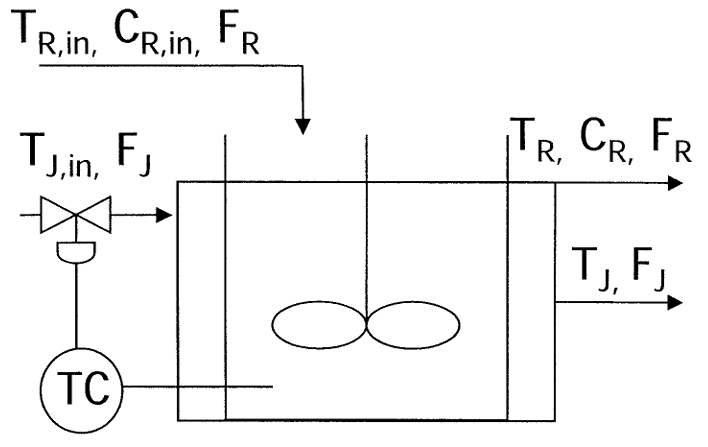
\includegraphics[width=0.8\textwidth]{CSTR.png}
    \caption{Illustration of the CSTR case.}
\end{figure}

% =========================================================
\section{Notation and Parameters}
\subsection{Time horizon and indices}
Continuous time horizon: $t \in [0,t_f]$.\\
Discrete grid (used in \cref{sec:discretization}): $t_k = k\,\Delta t$, $k=0,1,\ldots,N$ with $\Delta t = t_f/N$.

\subsection{Geometry} \label{subsec:geometry}
Reactor volume and area (function of design parameters $D_R$ and $H_R$):
\begin{align}
    V_R &= \frac{\pi}{4}\,D_R^2 H_R, & A_R &= \pi D_R H_R.
\end{align}

\subsection{Model variables and parameters}
\begin{table}[H]
\centering
\caption{Decision variables (continuous-time).}
\label{tab:variables}
\begin{tabularx}{\textwidth}{@{}lXl@{}}
\toprule
\textbf{Symbol} & \textbf{Meaning} & \textbf{Bounds / Units}\\
\midrule
$C_R(t)$ & Reactant concentration in reactor & $0 \le C_R \le C_{R,in}$ \;(\si{mol.{A/m^{3}}})\\
$T_R(t)$ & Reactor temperature & $T_{R,\min} \le T_R \le T_{R,\max}$ \;(\si{K})\\
$T_J(t)$ & Jacket temperature & $T_{J,\min} \le T_J \le T_{J,\max}$ \;(\si{K})\\
$F_J(t)$ & Jacket flow rate (control) & $F_{J,\min} \le F_J \le F_{J,\max}$ \;(\si{m^{3}/hr})\\
$s_{\mathrm{conv}}(t)$ & Slack for conversion constraint & $s_{\mathrm{conv}} \ge 0$\\
$s_{\mathrm{cool}}(t)$ & Slack for cooling/heat duty constraint & $s_{\mathrm{cool}} \ge 0$\\
$s_{\mathrm{temp}}(t)$ & Slack for temperature gradient constraint & $s_{\mathrm{temp}} \ge 0$\\[2pt]
\bottomrule
\end{tabularx}
\end{table}

\begin{table}[H]
\centering
\caption{Model parameters.}
\label{tab:parameters}
\begin{tabularx}{\textwidth}{@{}lXl@{}}
\toprule
\textbf{Symbol} & \textbf{Meaning} & \textbf{Units}\\
\midrule
$D_R$ & Reactor diameter (design) & \si{m}\\
$H_R$ & Reactor height (design) & \si{m}\\
$k_0$ & kinetic rate constant & \si{hr^{-1}}\\
$E_a/R$ & Activation energy & \si{K}\\
$\Delta H$ & Heat of reaction & \si{KJ/mol}\\
$\rho, C_p$ & Reactor liquid density, heat capacity & \si{kg/m^{3}}, \si{kJ/kg.K}\\
$\rho_J, C_{p,J}$ & Jacket liquid density, heat capacity & \si{kg/m^{3}}, \si{kJ/kg.K}\\
$U, A_R$ & Overall heat transfer coeff. and area & \si{{kJ/hr}.m^{2}.K}, \si{m^2}\\
$V_R(V_J)$ & Reactor(Jacket) volume & \si{m^{3}}\\
$F_R(F_J)$ & Reactor(Jacket) feed volumetric flow rate & \si{m^{3}/hr} \\
$C_{R,in}$ & Inlet reactant concentration & \si{mol.{A/m^{3}}}\\
$T_{R,in}, T_{J,in}$ & Inlet temperatures (reactor feed, jacket) & \si{K}\\
\addlinespace[2pt]
\multicolumn{3}{@{}l}{\textit{Operational parameters}}\\
$T_{R,\min}, T_{R,\max}$ & Reactor temperature bounds & \si{K}\\
$T_{J,\min}, T_{J,\max}$ & Jacket temperature bounds & \si{K}\\
$F_{J,\min}, F_{J,\max}$ & Jacket flow bounds & \si{m^{3}.h^{-1}}\\
$C_{R,0}, T_{R,0}, T_{J,0}$ & Initial concentration and temperatures & $\si{mol.{A/m^{3}}}$\\
\addlinespace[2pt]
$X_{\min}$ & Minimum required conversion & --\\
$Q_{\max}$ & Max cooling/heat duty allowance & \si{W}\\
$\Delta T_{\max}$ & Max allowed temperature change rate & \si{K/hr}\\
\addlinespace[2pt]
$P_{\mathrm{prod}}$ & Product price & \si{\$/mol}\\
$P_{\mathrm{react}}$ & Reactant cost & \si{\$/mol}\\
$P_{\mathrm{energy}}$ & Energy cost (cooling/heating) & \si{\$/kJ}\\
% $P_{\mathrm{op}}$ & Operating cost density (per reactor volume) & \si{\$/m^{3}}\\
$w_{\mathrm{conv}}$ & Penalty weight for conversion slack & \si{\$/(\text{unit})}\\
$w_{\mathrm{cool}}$ & Penalty weight for cooling slack & \si{\$/(\text{unit})}\\
$w_{\mathrm{temp}}$ & Penalty weight for temperature ramp slack & \si{\$/(\text{unit})}\\
\bottomrule
\end{tabularx}
\end{table}

% =========================================================
\section{Continuous-Time Model}
\subsection{Reaction kinetics}
\begin{equation}
    k(t) = k_0 \exp\!\left(-\frac{E_a}{R\,T_R(t)}\right).
\end{equation}

\subsection{Mass balance}
\begin{equation}
    \frac{d C_R}{dt} = \frac{F_R}{V_R}\,\big(C_{R,in} - C_R\big) - k\,C_R.
\end{equation}

\subsection{Energy balances}
\paragraph{Reactor.}
\begin{equation}
    \frac{d T_R}{dt}
    = \frac{F_R}{V_R}\,\big(T_{R,in} - T_R\big)
      - \frac{\Delta H}{\rho C_p}\,k\,C_R
      - \frac{U A_R}{\rho C_p V_R}\,\big(T_R - T_J\big).
\end{equation}

\paragraph{Jacket.}
\begin{equation}
    \frac{d T_J}{dt}
    = \frac{F_J}{V_J}\,\big(T_{J,in} - T_J\big)
      + \frac{U A_R}{\rho_J C_{p,J} V_J}\,\big(T_R - T_J\big).
\end{equation}

\section{Operational Constraints (Continuous-time)}
\paragraph{Box bounds.} As listed in \cref{tab:variables} and \cref{tab:parameters}.

\paragraph{Temperature change (soft).} The absolute change is limited with a nonnegative slack:
\begin{equation}
    \left|\frac{dT_R}{dt}\right| \le \Delta T_{\max} + s_{\mathrm{temp}}(t), \qquad s_{\mathrm{temp}}(t) \ge 0.
\end{equation}

\paragraph{Conversion (soft).}
\begin{equation}
    {C_{R,in} - C_R(t)} + s_{\mathrm{conv}}(t) \ge X_{\min}, \qquad s_{\mathrm{conv}}(t) \ge 0.
\end{equation}

\paragraph{Cooling/heat duty (soft).}
\begin{equation}
    U A_R \,\big|T_R(t) - T_J(t)\big| \le Q_{\max} + s_{\mathrm{cool}}(t), \qquad s_{\mathrm{cool}}(t) \ge 0.
\end{equation}

\paragraph{Initial conditions.}
can be set from the environment/plant measurements.
\begin{equation}
    C_R(0) = C_{R,0}, \quad T_R(0) = T_{R,0}, \quad T_J(0) = T_{J,0}.
\end{equation}

% \section{Economic Objective (Continuous-time)}
% Maximize net profit over $[0,t_f]$, penalizing violations:
% \begin{align}
% \max \; & \int_0^{t_f} \Big(
%     P_{\mathrm{prod}}\,F_R\,(C_{R,in} - C_R)
%     - P_{\mathrm{energy}}\,U A_R\,\lvert T_R - T_J\rvert
% \Big)\,dt \nonumber\\
% & \quad - \int_0^{t_f} \big(
%       w_{\mathrm{conv}}\,s_{\mathrm{conv}}
%     + w_{\mathrm{cool}}\,s_{\mathrm{cool}}
%     + w_{\mathrm{temp}}\,s_{\mathrm{temp}}
% \big)\,dt
% \end{align}
% subject to the dynamic model and constraints above.

% =========================================================
\section{Backward-Euler Discretization and Discrete Model} \label{sec:discretization}
Let $k=1,\dots,N$ with $t_k = k\,\Delta t$. Denote $C_{R,k}\approx C_R(t_k)$ (similarly for $T_{R,k}$, $T_{J,k}$, slacks and controls). Backward–Euler for any state $x$ reads
\begin{equation}
    \left.\frac{dx}{dt}\right|_{t=t_k} \approx \frac{x_k - x_{k-1}}{\Delta t}.
\end{equation}

\subsection{Discrete variables (per time step $k$)}
States: $C_{R,k},\,T_{R,k},\,T_{J,k}$; Manipulated variable: $F_{J,k}$; Slacks: $s_{\mathrm{conv},k},\,s_{\mathrm{cool},k},\,s_{\mathrm{temp},k}$.

\subsection{Discrete kinetics}
\begin{equation}
    k_k = k_0 \exp\!\left(-\frac{E_a}{R\,T_{R,k}}\right).
\end{equation}

\subsection{Discrete dynamics (Backward–Euler)}
\begin{align}
    C_{R,k} &= C_{R,k-1} + \Delta t \left[\frac{F_R}{V_R}(C_{R,in} - C_{R,k}) - k_k C_{R,k}\right], \\
    T_{R,k} &= T_{R,k-1} + \Delta t \Big[
        \frac{F_R}{V_R}(T_{R,in} - T_{R,k})
        - \frac{\Delta H}{\rho C_p} k_k C_{R,k}
        - \frac{U A_R}{\rho C_p V_R}(T_{R,k} - T_{J,k})
    \Big],\\
    T_{J,k} &= T_{J,k-1} + \Delta t \Big[
        \frac{F_{J,k}}{V_J}(T_{J,in} - T_{J,k})
        + \frac{U A_R}{\rho_J C_{p,J} V_J}(T_{R,k} - T_{J,k})
    \Big].
\end{align}

\subsection{Discrete constraints}
\paragraph{bounds.}
\begin{align}
    0 \le &\, C_{R,k} \le C_{R,in}, &
    T_{R,\min} \le &\, T_{R,k} \le T_{R,\max}, &
    T_{J,\min} \le &\, T_{J,k} \le T_{J,\max},\\
    F_{J,\min} \le &\, F_{J,k} \le F_{J,\max}, &
    s_{\mathrm{conv},k}, s_{\mathrm{cool},k}, s_{\mathrm{temp},k} &\ge 0.
\end{align}

\paragraph{Temperature ramp (soft).}
\begin{equation}
    -\Delta T_{\max} - s_{\mathrm{temp},k}
    \;\le\; {T_{R,k} - T_{R,k-1}}
    \;\le\; \Delta T_{\max} + s_{\mathrm{temp},k}.
\end{equation}

\paragraph{Conversion (soft).}
\begin{equation}
    {C_{R,in} - C_{R,k}} + s_{\mathrm{conv},k} \ge X_{\min}.
\end{equation}

\paragraph{Cooling/heat duty (soft).}
\begin{equation}
    U A_R \,\lvert T_{R,k} - T_{J,k}\rvert \le Q_{\max} + s_{\mathrm{cool},k}.
\end{equation}

\paragraph{Initial conditions.}
\begin{equation}
    C_{R,0} = C_{R,0}^{\text{given}}, \quad
    T_{R,0} = T_{R,0}^{\text{given}}, \quad
    T_{J,0} = T_{J,0}^{\text{given}}.
\end{equation}

\subsection{Discrete economic objective}
\begin{align}
\max \; & \sum_{k=1}^N \Delta t \,\Big(
    P_{\mathrm{prod}}\,F_R\,(C_{R,in} - C_{R,k})
    % - P_{\mathrm{react}}\,F_R\,C_{R,in}
    - P_{\mathrm{energy}}\,U A_R\,\lvert T_{R,k} - T_{J,k}\rvert
\Big) \nonumber\\[-2pt]
& \quad - \sum_{k=1}^N \Delta t \,\big(
      w_{\mathrm{conv}}\,s_{\mathrm{conv},k}
    + w_{\mathrm{cool}}\,s_{\mathrm{cool},k}
    + w_{\mathrm{temp}}\,s_{\mathrm{temp},k}
\big).
\end{align}

% =========================================================
\section{Two-Layer RL-DRTO Architecture}
\subsection{Purpose and role}
The upper layer solves the discrete DRTO problem to compute an economically optimal reactor temperature setpoint trajectory. For online use, we pass a terminal or receding-horizon setpoint to the lower layer. In the RL variant, a trained policy directly maps measurements to safe setpoints without online optimization.

\subsection{Setpoint handoff}
After solving the DRTO over $k=0..N$, pass
\begin{equation}
    T_{R,sp} = T_{R,N}^{*}.
\end{equation}
Alternatively, use a policy $\pi_\theta$:
\begin{equation}
    T_{R,sp} = \pi_{\theta}(s_k), \qquad s_k = [T_R, T_J, e_k, F_J, \ldots].
\end{equation}

\subsection{Environment: PI-controlled CSTR (updated dynamics)}
The environment represents the plant dynamics; the PI controller tracks $T_{R,sp}$.
\begin{align}
V_R\,\frac{dC_R}{dt} &= F_R\,C_{R,in} - F_R\,C_R - k(t)\,V_R\,C_R, \\
V_R\,\frac{dT_R}{dt} &= F_R\,T_{R,in} - F_R\,T_R - \frac{\Delta H}{\rho C_p}\,k(t)\,V_R\,C_R - \frac{U}{\rho C_p}\,A_R\,(T_R - T_J), \\
V_J\,\frac{dT_J}{dt} &= F_J\,T_{J,in} - F_J\,T_J + \frac{U}{\rho_J C_{p,J}}\,A_R\,(T_R - T_J),
\end{align}
with $k(t) = k_0 \exp(-E_a/(R T_R))$.

\subsection{PI controller}
Let $e(t) = T_{R,sp} - T_R(t)$. Discrete incremental form:
\begin{align}
\Delta u_k &= K_c \Big[e_k - e_{k-1} + \frac{\Delta t}{\tau_I} e_k \Big], \\
F_J^k &= F_J^{k-1} + \Delta u_k, \qquad F_{J,\min} \le F_J^k \le F_{J,\max}.
\end{align}

\subsection{RL observations and reward}
\begin{align}
s_k &= [T_R, T_J, e_k, F_J], \\
r_k &= P_{\mathrm{prod}} F_R (C_{R,in} - C_R) - P_{\mathrm{energy}} U A_R |T_R - T_J| - \lambda_1 (T_R - T_{R,sp})^2.
\end{align}

\subsection{Execution loop}
\begin{enumerate}[label=(\arabic*)]
  \item DRTO/RL computes $T_{R,sp}$ every $\Delta t_{\mathrm{RTO}}$.
  \item PI adjusts $F_J$ to track $T_{R,sp}$.
  \item Plant evolves under the continuous dynamics.
  \item Measurements feed back to the DRTO/RL layer.
\end{enumerate}

% % =========================================================
% \section{Scaling and Numerical Notes}
% \begin{itemize}[leftmargin=1.25em]
%     \item State scaling: $\hat{C}_R = C_R/C_{R,in}$, $\hat{T}_R = T_R/T_{R,\max}$, $\hat{T}_J = T_J/T_{J,\max}$.
%     \item Residual scaling: multiply dynamic residuals by $\Delta t$ to improve conditioning.
%     \item Economic scaling: divide objective terms by a nominal production value.
%     \item Slacks: initialize $s_{\mathrm{conv},k}$, $s_{\mathrm{cool},k}$, $s_{\mathrm{temp},k}$ with small positive values (e.g., $10^{-5}$).
% \end{itemize}

% =========================================================
\section{Notes on Dynamics Placement}
All physical plant dynamics reside in the lower (environment) layer. The upper DRTO layer contains a predictive model used for optimization, here discretized by backward–Euler. An RL policy can replace repeated online optimization by directly mapping observed states to safe setpoints.

\end{document}
